\section{Диаграммы Вороного}

    \begin{frame}{Диаграмма Вороного}

        \begin{defn}

            Пусть $S$~--- конечное подмножество $\mathbb{R}^2$ (его точки~--- \alert{сайты}).
            Диаграммой Вороного $\mathcal{V}\mathcal{D}(S)$ называется разбиение плоскости на $n$ ячеек $\{ F_i \}$, при котором $x \in F_i
            \Leftrightarrow s_i \in S$~--- ближайший к $x$ \alert{сайт}.

        \end{defn}

        Мы рассматриваем $\mathcal{V}\mathcal{D}(S)$ в рамках ограниченной области плоскости, содержащей все её
        вершины.

    \end{frame}

    \begin{frame}{Диаграмма Вороного}
        
        \begin{center}

            \resizebox{0.5\columnwidth}{!}{\incfig{VD_0}}

        \end{center}

        
    \end{frame}

    \begin{frame}{Post office problem}
    \vspace{-17.5mm}
    \begin{center}

        \resizebox{0.75\columnwidth}{!}{\incfig{Post_Office}}

    \end{center}

    \end{frame}

    \begin{frame}{Свойства диаграмм Вороного}

        \begin{itemize}

            \item Cерединный перпендикуляр к $s_i s_j$ делит плоскость на две гиперплоскости. Пусть $H(s_i s_j)$~--- та из них, которая содержит $s_i$.
                  Тогда
                  \[ F_i = \bigcap\limits_{j = 1, \ j \neq i}^{n} H(s_i, s_j)\]

            \item Вершина~--- центр окружности, проходящей через 3 соседних с ней сайта.

            \item Клетка сайта $s_i$ неограничена $\Leftrightarrow s_i \in \mathcal{C}\mathcal{H}(S)$.

        \end{itemize}

    \end{frame}

    \begin{frame}{Свойства диаграмм Вороного}

        \begin{itemize}

            \item $\mathcal{V}\mathcal{D}(S)$~--- планарный трёхсвязный 3-регулярный граф.

            \item Удобно хранить в $DCEL$.

            \item Если $|S| = n$, то $V(\mathcal{V}\mathcal{D}(S)) \le 2n - 5$, $E(\mathcal{V}\mathcal{D}(S)) \le 3n - 6$.

            \item Занимает линейный размер по памяти.

        \end{itemize}
    \end{frame}

    \begin{frame}{Построение диаграммы Вороногго: Brute force}

        \alert{Идея:} пересекать серединные перпендикуляры.

        Построение ячейки для сайта $s_i$:

        \begin{enumerate}
            \item Проводим все серединные перпендикуляры между $s_i$ и $s_j$, $i \neq j$.

            \item Пересекаем попарно все серединные перпендикуляры,\\ получаем $O(n^2)$ точек.

            \item Каждую проверяем на принадлежность каждой из\\ $n - 1$ полуплоскостей.

        \end{enumerate}

        Время работы: $T(n) = n \cdot O(n^2) \cdot (n - 1) = O(n^4)$.

    \end{frame}

    \begin{frame}{Построение $\mathcal{V}\mathcal{D}(S)$: Пересечение полуплоскостей}

        Рассмотрим теперь более быстрый алгоритм, использующий геометрические идеи, связанные с пересечением полуплоскостей. \\

        Сначала мы реализуем несколько важных процедур, а после научимся более оптимально пересекать полуплоскости.

    \end{frame}

    \begin{frame}{Принадлежность точки выпуклому многоугольнику}

        \begin{itemize}

            \item Пускаем луч из точки в произвольном направлении.

            \item Если он пересекает границу многоугольника нечетное число раз, то точка внутри.
                  Если четное~--- снаружи.

        \end{itemize}

        \begin{center}
        \begin{tikzpicture}[scale = 0.4]
        % polygon
        \coordinate (a) at (0,0); \coordinate (b) at (2, 4); \coordinate (c) at (4, 1); \coordinate (d) at (4, 7); \coordinate (e) at (11, 7); \coordinate (f) at (7, 3); \coordinate (g) at (13, 3); \coordinate (h) at (15, 5); \coordinate (i) at (21, 1); \coordinate (j) at (15, 2); \coordinate (k) at (13, 0);
        \draw[fill4, fill = fill4] (a) circle (0.07); \draw[fill4, fill = fill4] (b) circle (0.07); \draw[fill4, fill = fill4] (c) circle (0.07); \draw[fill4, fill = fill4] (d) circle (0.07); \draw[fill4, fill = fill4] (e) circle (0.07); \draw[fill4, fill = fill4] (f) circle (0.07); \draw[fill4, fill = fill4] (g) circle (0.07); \draw[fill4, fill = fill4] (h) circle (0.07); \draw[fill4, fill = fill4] (j) circle (0.07); \draw[fill4, fill = fill4] (k) circle (0.07);
        % dots
        \coordinate (x) at (2, 1); \coordinate (y) at (11, 5);
        \draw[fill5, fill = fill5] (x) circle (0.07); \draw[fill5, fill = fill5] (y) circle (0.07);
        \draw[fill5, fill = fill5] (0, 2) circle (0.07); \draw[fill5, fill = fill5] (8, 8) circle (0.07); \draw[fill5, fill = fill5] (15, 0) circle (0.07);

        \draw[fill5, dashed, thick] (x)--(0, 2);
        \draw[fill5, dashed, thick] (x)--(8, 8);
        \draw[fill5, dashed, thick] (y)--(15, 0);

        \draw[fill4, fill=fill4, fill opacity=0.5, draw opacity = 0] (a)--(b)--(c)--(d)--(e)--(f)--(g)--(h)--(i)--(j)--(k)--cycle;

        \end{tikzpicture}
        \end{center}

    \end{frame}

    \begin{frame}{Пересечение выпуклых многоугольников}

        Пользуясь предыдущей процедурой, работающей за $O(n)$ \\ (и $O(\log(n)$ на выпуклом), получаем наивный алгоритм:

        \begin{itemize}
		\item Пересекаем каждую сторону первого многоугольника \\ с каждой стороной второго: получаем \\ \(O \lr*{m} \) точек \(I_{e_i, \epsilon_j}\) (макс. две на ребре), \\ которые будут вершинами пересечения.
		\end{itemize} \end{frame}

\begin{frame}{Пересечение выпуклых многоугольников}
		\begin{itemize}
		\item Надо отсортировать \(I_{e_i, \epsilon_j}\) и вершины по аргументу относительно какой-либо точки пересечения (например, одной из них).
		\[O \lr*{\lr*{m+n} \cdot \log \lr*{m+n}} .\]

		\item Из упорядоченного набора точек надо выкинуть не-вершины.\\
		Для этого проверяем {\it вершины многоугольников} (\(I_{e_i, \epsilon_j}\) не надо)\\
		на принадлежность {\it обоим} многоугольникам.
		\[O \lr*{\lr*{m+n} \cdot \lr*{\log m + \log n}} .\]
        \end{itemize}
    \end{frame}

    \begin{frame}{Пересечение вып. многоугольников: O'Rourke}

        \begin{itemize}

            \item Вершины многоугольников упорядочены против часовой стрелки.

            \item Движемся по границам и на каждом шаге определяем, по какому многоугольнику переходить на одну вершину дальше.

        \end{itemize}

        \begin{center}
        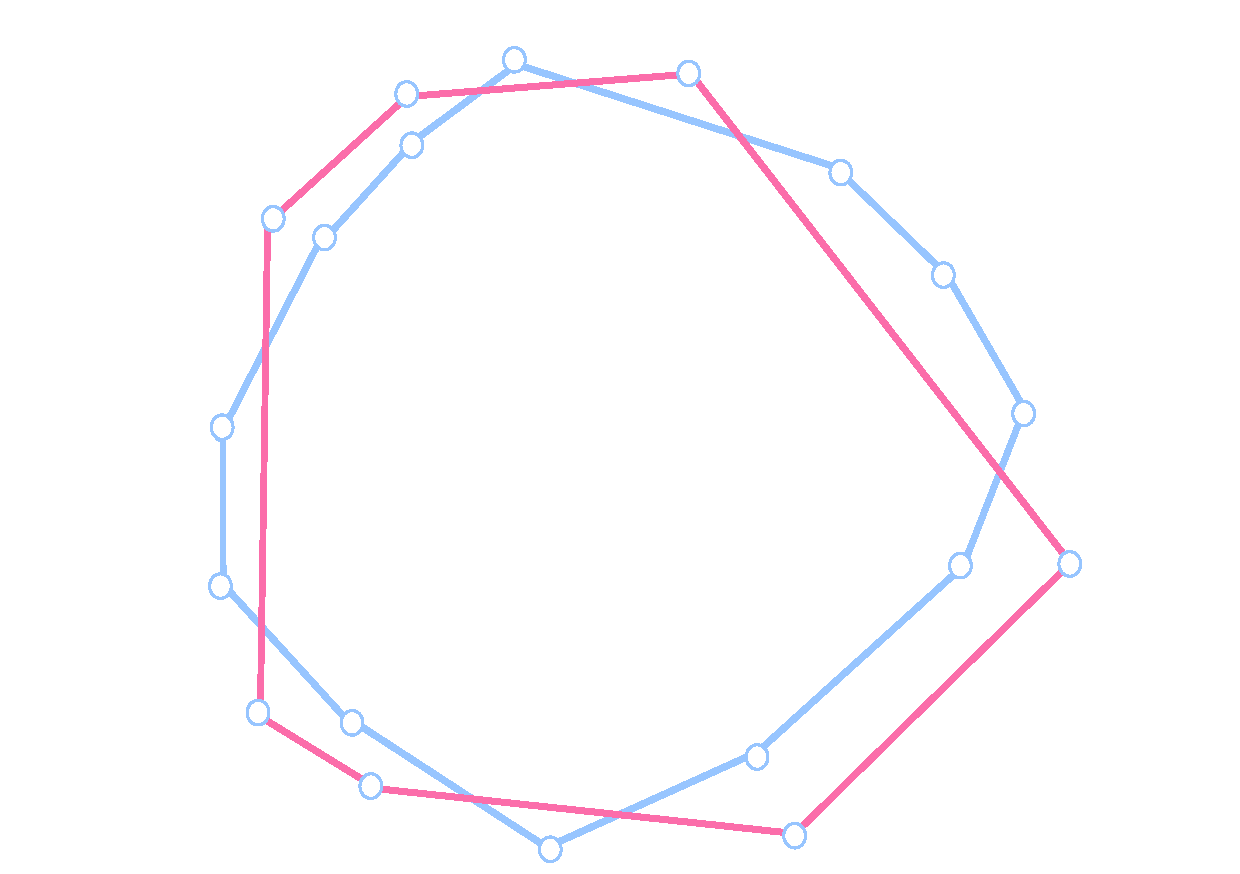
\includegraphics[width=0.42\textwidth]{картинки/пересечение_мн-в.pdf}
        \ \ 
        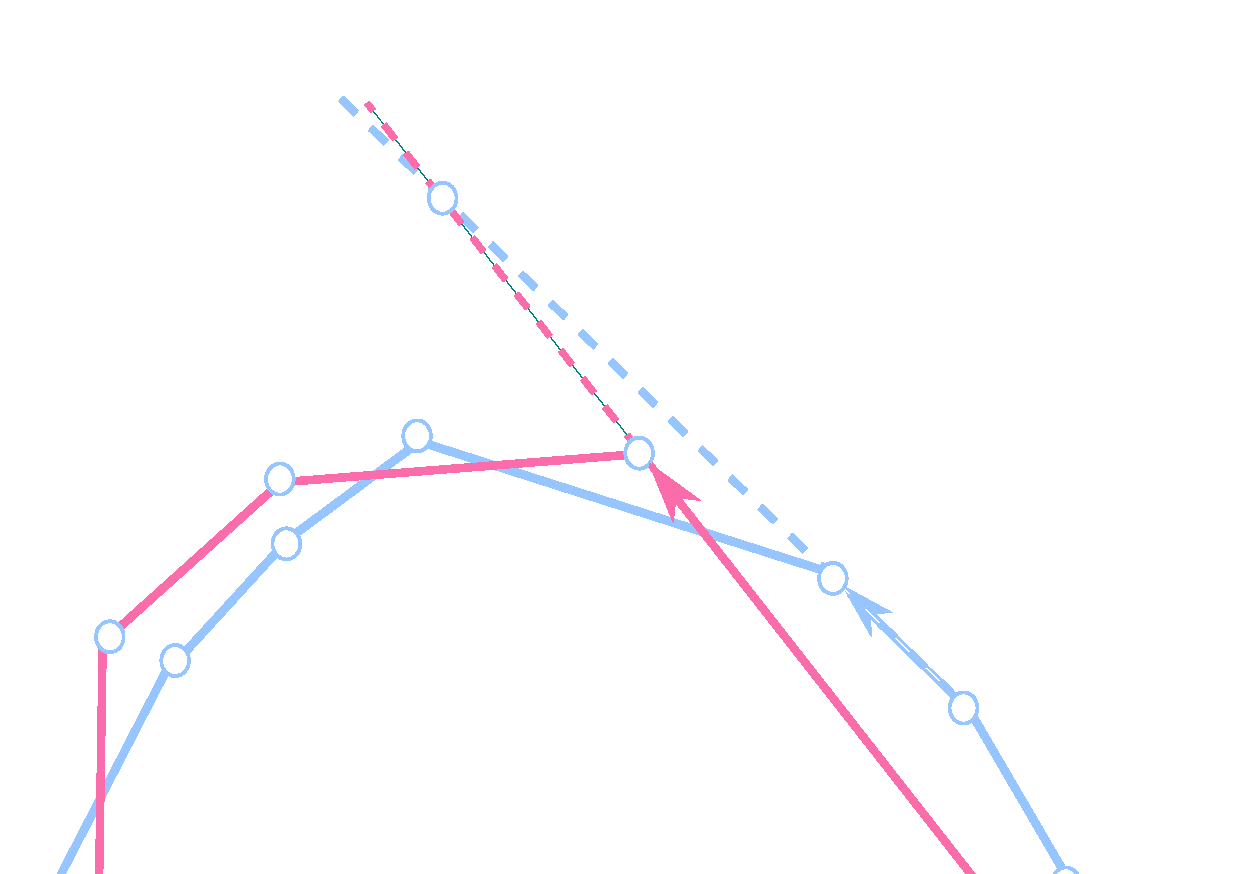
\includegraphics[width=0.42\textwidth]{картинки/крупное_пересечение_мн-в.pdf}
        \end{center}

    \end{frame}


    \begin{frame}{Пересечение вып. многоугольников: O'Rourke}

        \begin{itemize}

            \item Каждый раз получаем одну из восьми ситуаций:

            \begin{center}
            \begin{tikzpicture}[scale = 0.5]
            \begin{scope}
            % first:
            \coordinate (a) at (0,0); \coordinate (b) at (3, 5); \coordinate (c) at (3, 0); \coordinate (d) at (0, 5); \coordinate (e) at (1.5, 2.5); \coordinate (f) at (0.64, 1.07); \coordinate (g) at (2.25, 1.25);
            \draw[fill5, fill = fill5] (a) circle (0.13); \draw[fill5, fill = fill5] (b) circle (0.13); \draw[fill4, fill = fill4] (c) circle (0.13); \draw[fill4, fill = fill4] (d) circle (0.13); \draw[fill5, fill = fill5] (f) circle (0.13); \draw[fill4, fill = fill4] (g) circle (0.13);
            \draw[fill5, thick] (a)--(b);
            \draw[fill4, thick] (c)--(d);
            \draw[fill5, thick, ->] (a)--(f);
            \draw[fill4, thick, ->] (c)--(g);
            \draw[fill3, fill=fill3, fill opacity=0.5, draw opacity = 0] (a)--(e)--(d)--cycle;
            \end{scope}
            \begin{scope}[xshift = 6.5cm]
            % second:
            \coordinate (a) at (0,0); \coordinate (b) at (3, 5); \coordinate (c) at (3, 0); \coordinate (d) at (0, 5); \coordinate (e) at (1.5, 2.5); \coordinate (f) at (2.25, 3.75); \coordinate (g) at (2.25, 1.25);
            \draw[fill5, fill = fill5] (a) circle (0.13); \draw[fill5, fill = fill5] (b) circle (0.13); \draw[fill4, fill = fill4] (c) circle (0.13); \draw[fill4, fill = fill4] (d) circle (0.13); \draw[fill5, fill = fill5] (f) circle (0.13); \draw[fill4, fill = fill4] (g) circle (0.13);
            \draw[fill5, thick] (a)--(b);
            \draw[fill4, thick] (c)--(d);
            \draw[fill5, thick, ->] (a)--(f);
            \draw[fill4, thick, ->] (c)--(g);
            \draw[fill3, fill=fill3, fill opacity=0.5, draw opacity = 0] (a)--(e)--(d)--cycle;
            \end{scope}
            \begin{scope}[xshift = 13cm]
            % third:
            \coordinate (a) at (0,0); \coordinate (b) at (3, 5); \coordinate (c) at (3, 0); \coordinate (d) at (0, 5); \coordinate (e) at (1.5, 2.5); \coordinate (f) at (0.64, 1.07); \coordinate (g) at (0.75, 3.75);
            \draw[fill5, fill = fill5] (a) circle (0.13); \draw[fill5, fill = fill5] (b) circle (0.13); \draw[fill4, fill = fill4] (c) circle (0.13); \draw[fill4, fill = fill4] (d) circle (0.13); \draw[fill5, fill = fill5] (f) circle (0.13); \draw[fill4, fill = fill4] (g) circle (0.13);
            \draw[fill5, thick] (a)--(b);
            \draw[fill4, thick] (c)--(d);
            \draw[fill5, thick, ->] (a)--(f);
            \draw[fill4, thick, ->] (c)--(g);
            \draw[fill3, fill=fill3, fill opacity=0.5, draw opacity = 0] (a)--(e)--(d)--cycle;
            \end{scope}
            \begin{scope}[xshift = 19.5cm]
            % second:
            \coordinate (a) at (0,0); \coordinate (b) at (3, 5); \coordinate (c) at (3, 0); \coordinate (d) at (0, 5); \coordinate (e) at (1.5, 2.5); \coordinate (f) at (2.25, 3.75); \coordinate (g) at (0.75, 3.75);
            \draw[fill5, fill = fill5] (a) circle (0.13); \draw[fill5, fill = fill5] (b) circle (0.13); \draw[fill4, fill = fill4] (c) circle (0.13); \draw[fill4, fill = fill4] (d) circle (0.13); \draw[fill5, fill = fill5] (f) circle (0.13); \draw[fill4, fill = fill4] (g) circle (0.13);
            \draw[fill5, thick] (a)--(b);
            \draw[fill4, thick] (c)--(d);
            \draw[fill5, thick, ->] (a)--(f);
            \draw[fill4, thick, ->] (c)--(g);
            \draw[fill3, fill=fill3, fill opacity=0.5, draw opacity = 0] (a)--(e)--(d)--cycle;
            \end{scope}
            \end{tikzpicture}
            \end{center}

            \item В случаях (1) и (2) двигаемся по второму многоугольнику, в случаях (3) и (4)~--- по первому. \\
                  Кроме того, для случая (4) необходимо вычислить и добавить точку пересечения.

        \end{itemize}
    \end{frame}


    \begin{frame}{Пересечение вып. многоугольников: O'Rourke}

        \begin{itemize}

            \item В результате полного обхода получаем точки пересечения. Если каждый раз будем брать ломаные, лежащие левее в порядке обохода, получим пересечение.

            \item Интересно, что если каждый раз будем брать лежащую правее~--- получим объединение.

        \end{itemize}

        Время работы: $T(n, m) \le 2(n + m) = O(n + m)$.
    \end{frame}
    

    \begin{frame}{Построение $\mathcal{V}\mathcal{D}(S)$: Пересечение полуплоскостей}

        Наконец, перейдем к построению диаграммы Вороного.

        \begin{itemize}

            \item Строим все серединные перпендикуляры к отрезкам, соединяющим сайт $s_i$ с остальными сайтами, получаем $n - 1$ полуплоскость.

            \item Пересекаем все полуплоскости следующим образом: \\
                  Сначала все пары, потом пары пересечений и так далее.

            \item Получаем клетку для выбранного сайта.

        \end{itemize}

        Время работы: $T(n) = O(n \cdot n \cdot \log(n)) = O(n^2 \log(n))$.

    \end{frame}

    \begin{frame}{Недостатки этих алгоритмов}

        \begin{itemize}

            \item Неоптимальное время работы~--- можно за  $O(n \log(n))$.

            \item На выходе получаем список клеток (без всякой информации о их взаимосвязях).

        \end{itemize}

        Решение: алгоритм Форчуна с использованием DCEL.\\

        Или алгоритм $D\&C$ за $O(n\log(n))$.

    \end{frame}

\section{Триангуляции Делоне}

    \begin{frame}{Триангуляция Делоне}

        \begin{defn}

            Пусть $S$~--- конечное подмножество $\mathbb{R}^2$.
            Триангуляцией Делоне  $\mathcal{D}\mathcal{T}(S)$  называется такая триунгуляция этого множества,
            при которой круг, описанный около каждого треугольника не содержит других вершин триангуляции.

        \end{defn}

    \end{frame}

    \begin{frame}{Триангуляция Делоне}
         \vspace{2mm}
         \begin{center}

            \resizebox{0.75\columnwidth}{!}{\incfig{DT_1}}

        \end{center}

    \end{frame}

    \begin{frame}{Триангуляция Делоне}
         \vspace{2mm}
         \begin{center}

            \resizebox{0.75\columnwidth}{!}{\incfig{DT_1.5}}

        \end{center}

    \end{frame}

\section{VD и DT — двойственные графы}

    \begin{frame}{$\mathcal{V}\mathcal{D}(S)$ и $\mathcal{D}\mathcal{T}(S)$~--- двойственные графы}

        \vspace{2mm}

        \begin{thm}

            $\mathcal{D}\mathcal{T}(S)$~--- двойственный граф к $\mathcal{V}\mathcal{D}(S)$.

        \end{thm}

        \begin{center}

            \resizebox{0.6\columnwidth}{!}{\incfig{VD_DT_Finally}}

        \end{center}

    \end{frame}

    \begin{frame}{$\mathcal{V}\mathcal{D}(S)$ и $\mathcal{D}\mathcal{T}(S)$~--- двойственные графы}

        \begin{proof}

            Рассмотрим сайты $s_i, s_j, s_k$ из одного треугольника в триангуляции Делоне. Тогда вершина диаграммы Вороного~---
            центр описанной окружности треугольника $\triangle s_i s_j s_k$.\\

            Так как центр описанной окружности единственный, мы получили взаимнооднозначное соответствие.

        \end{proof}

    \end{frame}

    \begin{frame}{$\mathcal{V}\mathcal{D}(S)$ и $\mathcal{D}\mathcal{T}(S)$~--- двойственные графы}

        \begin{block}{Следствие}

                При условии общего положения триангуляция Делоне \\ множества точек единственна.

        \end{block}

        То есть, если мы умеем строить диаграмму Вороного и храним её в DCEL, то мы умеем строить и триангуляцию
        Делоне.

    \end{frame}

    \begin{frame}{Свойства триангуляции Делоне}

        \begin{itemize}

            \item Максимизирует минимальный угол.

            \item $MST$~--- подграф триангуляции Делоне (что позволяет относительно эффективно его считать).

            \item Так как триангуляция Делоне избегает узких (похожих на вырожденные) треугольников, её часто использвют
                  в самом разнои моделировании. Например, ландшафтном.

        \end{itemize}

    \end{frame}
